\documentclass[anon]{CI}
\usepackage[latin1]{inputenc}
\usepackage[english]{babel}
\usepackage[]{algorithm2e}
\usepackage{algorithmic}


% The following packages will be automatically loaded:
% amsmath, amssymb, natbib, graphicx, url, algorithm2e

\title[CI Project]{Swarm intelligence for counting the degrees of separation in Social Networks}

 % Use \Name{Author Name} to specify the name.
 % If the surname contains spaces, enclose the surname
 % in braces, e.g. \Name{John {Smith Jones}} similarly
 % if the name has a "von" part, e.g \Name{Jane {de Winter}}.
 % If the first letter in the forenames is a diacritic
 % enclose the diacritic in braces, e.g. \Name{{\'E}louise Smith}

 % Two authors with the same address
  % \coltauthor{\Name{Author Name1} \Email{abc@sample.com}\and
  %  \Name{Author Name2} \Email{xyz@sample.com}\\
  %  \addr Address}

 % Three or more authors with the same address:
 % \coltauthor{\Name{Author Name1} \Email{an1@sample.com}\\
 %  \Name{Author Name2} \Email{an2@sample.com}\\
 %  \Name{Author Name3} \Email{an3@sample.com}\\
 %  \addr Address}


 % Authors with different addresses:
 \author{\Name{�lex Pardo Fernandez} \Email{alexpardo.5@gmail.com}\\
 \AND
 \Name{David S�nchez Pinsach} \Email{sdividis@gmail.com}\\
 }

\begin{document}

\maketitle

\begin{abstract}
This is a great project and therefore it has a concise abstract.
\end{abstract}

\begin{keywords}
Swarm Intelligence, Ant Colony Optimization, Twitter, Degrees of Separation.
\end{keywords}


\section{Problem statement and goals} % 1 p�gina

%\textbf{This is where the content of your paper starts. Remember:
%\begin{itemize}
%\item Limit the main text (without bibliography and appendices) to 10 pages.
%\item Include, either in the main text or the appendices, enough details to convince the lecturers of the project's merits.
%\item You should cite all relevant references, including your own.
%\end{itemize}}
\par
One of the most important features of humans and in general, of lots of animals, is the sociability. The ability of communicating each other in order to share knowledge. Human social relationships form a network where everyone is connected with those that communicates often (considered as friends). 
\\ \par
The theory of the six degrees of separation was originally set out by Frigyes Karinthy \citep{karinthy1929chain} and explains that everyone is connected to any other person in the world by six degrees. That means, if you want to met someone in the world, you will need to pass by other five persons, as maximum, between you and your objective so the last one will be the one you are trying to reach. During these last decades, the six degree theory has been used in many fields like economy, social networks and markets and is a known property of small-world networks where most nodes are not neighbours of one another, but most nodes can be reached from every other by a small number of steps.
\\\par
Twitter is one of the biggest social networks, that is over 200 million users and over 400 million tweets (the 140 character messages that are the main feature of this social network) every day \footnote{Information by March of 2013: \href{https://blog.twitter.com/2013/celebrating-twitter7}{https://blog.twitter.com/2013/celebrating-twitter7}}. The main idea is to create shorts messages of the 140 characters in order to express your ideas or opinions in a shorten way. Moreover, Twitter have introduced some concepts that are very popular now such as the \emph{hash-tag} which is a way of tagging the messages i order to find all the related ones.

%Another famous social network is Foursquare, a social network related to places in which you activate the application and notifies your friends that you have been in that place. The most active users in one place achieve some goals such as being the ``major'' of a certain place. Foursquare has over 45 million users and over 3 billion check-ins every day \footnote{Information by January of 2014: \href{https://foursquare.com/about}{https://foursquare.com/about}}.
We also used another dataset acquired from BlogCatalog, a social blog directory which manages the bloggers and their blogs. In this case, the edges are the friendships among the bloggers. The dataset we have has 10K nodes and over 300K edges and is available on \citep{ZafaraniLiu}.
\\\par
The main objective of this work will be to estimate the degrees of separation in BlogCatalog and if it is computationally possible, in Twitter and see if it is possible to obtain six degrees of separation between two random people. In order to do this task, it will use some ideas of the Computational Intelligence like Swarm Intelligence. In particular we are going to use Ant Colony Optimization (ACO) \citep{Colorni91} for Shortest Path finding (SPACO) \citep{angus}.



%Content:
%\begin{enumerate}
%\item Explain theory of the 6 degrees
%\item Define the network
%\item Goals: estimate the degrees of separation in twitter
%\end{enumerate}



\section{Previous work} % 2 p�gines

The previous work is based on these ideas:
\begin{itemize}
\item ACO original \citep{Colorni91}: Explain the algorithm of the Ant Colony Optimization.
\item General theory \citep{watts}: Explain the general theory about the six degree.
\item On Twitter as \citep{cheng}: Explain the six degree on the Twitter network.


\end{itemize}

\section{The CI methods} % 3-4 p�gines

Swarm intelligence is a natural method based in the behaviour of the decentralized individuals who obtain solutions in some problem as result of their interactions. These agents normally are simple, with a few capabilities and follow simple rules. It includes ACO, flocking of the birds, bacterial grow or some on. 
\\\\
As it is mentioned previously, we will use the ACO algorithm in order to obtain the degree of separation of two random person in a graph. This algorithm is inspired on the way ants have to solve the problem of finding the best path to achieve a goal such as going from the nest to the found food. The ants cannot communicate with the others and only use the trace of pheromone as a probabilistic method in order to obtain the choice when they have different options. When a ant travels through two points it leaves a few of pheromone on the trail. The other ants around these points feel the pheromone and try to follow this path. The paths with few pheromone will have less probability than the path with high pheromone. As shows the figure \ref{fig:aco}, the path of the ants converge to the shortest path between two points and this is the main characteristic of this method. We will use this idea of the shortest path between two points, as a minimum degree between two person in Foursquare and Twitter networks. In the appendix \ref{implementation}, it will be shown how the algorithm works in details.

\begin{figure}[htb!]
\centering
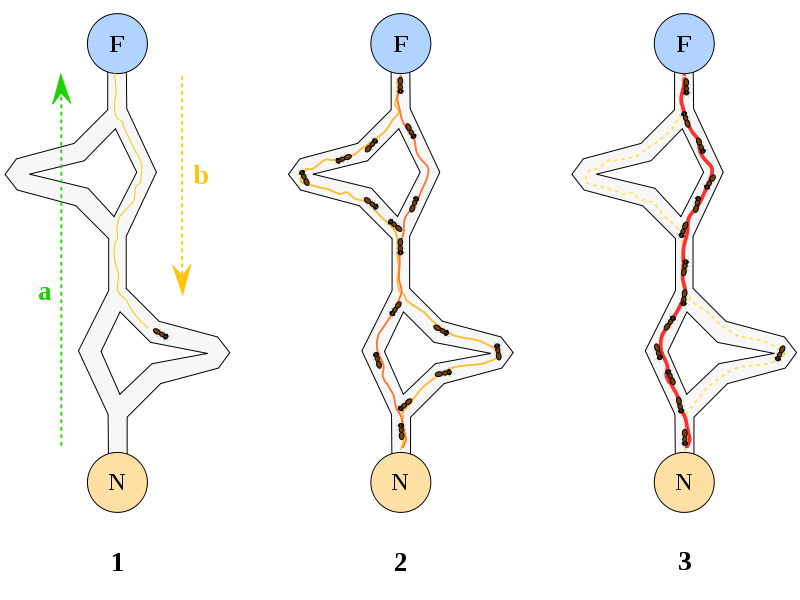
\includegraphics[width=0.6\textwidth]{img/aco}
\caption[ACO algorithm]{ACO algorithm\protect\footnote{Credits to Johann Dr�o, 27 may 2006}}
\label{fig:aco}
\end{figure}

Some considerations needed to take into account are the parameters of the algorithm. These are: the amount of pheromone leaved by each ant, the number of ants of the system, the dissipation of the pheromone and the number of epochs the algorithm will run.

% Amount of pheromone
% - set to 1
% - since weights are always 1, the pheromone is always the same
% - ants returning to the nest (start) leave pheromone also in the trail
% - additionally as \citep{dorigo1999ant} says, the amount of pheromone of the system is kept fixed, so at each iteration it is normalized to always sum a value equal to the number of nodes.


% Number of ants in the system
% - on each epoch, some ants are introduced on the system this allows the new ants to follow the paths started by the ants on the previous epochs
% - as \citep{dorigo1999ant} says, the number of ants should be equal to the number of nodes. Not possible in big graphs such as the Foursquare one, so we reduced the number of ants and increased the number of epochs
% - Once an ant is at distance 15 from the nest, we consider the ant has been lost so we do not follow it anymore (i.e. the ant is deleted from the system) this allows the code to run much more faster since we are only interested in shortest paths.

% Dissipation of the pheromone
% - disipation of pheromone allows the system to forget bad solutions in essence, bad solutions are long so the ants take longer to go from the nest to the food, the disipation allows the ants to explore aditional paths. Shortest paths also suffer the disipation but since are shorter, ants will arrive faster and the disipation will be compensated by the pheromone leaved

% Number of epochs
% - the number of epochs has to be taken into account using the number of ants on the system, the expected lentgh of the path and the computational time associated to the problem.
% - num of ants -> if there are a lot of ants, the system will be slower but will converge earlier, if the number of ants is lower, we will have to increase the number of epochs in order to converge
% - expected length of the path -> the number of epochs is expected to be greatest than the expected length of the shortest path since ants perform one step at each epoch.
% - Computational time -> since we are working with huge graphs (3 million of nodes and 11 million of edges), the computational cost of the algorithm is crucial, and the greatest the number of epochs, the greatests the number of expaned nodes. As explained on \ref{implementation}, the pheromones saved are the ones in which the amount is increased, so when the number of expanded nodes increasesm the ammount of memory needed also increases.

\section{Results and Discussion} % 1-2 p�gines de text

In order to perform the tests we used three different datasets. The first ones are a subset of Twitter network. The third one has been obtained from \citep{ZafaraniLiu} and is based on BlogCatalog network.
\par
Each dataset has been used changing the parameters of the algorithm in order to get the shortest path using the less computational resources. This parameters have been experimentally set.

\begin{table}
\centering
\begin{tabular}{l|l}
\hline
NUM\_ANTS & Maximum number of the ants in the system \\ \hline
ITERATIONS & Number of the experiments \\ \hline
DECAY & Factor of evaporation of the pheromones \\ \hline
INCREMENT & Number of the increment of the pheromones \\ \hline
ANTS\_PER\_TURN & Number of ants at each turn that appears \\ \hline
MAX\_EPOCH & Number of the iterations at each experiment \\ \hline
\end{tabular}
\caption{Table of the parameters description of the algorithm}
\label{parameters}
\end{table}

The next table \ref{datasets}, shows the number of the nodes and edges at each dataset.
\begin{table}[htb!]
\centering
\begin{tabular}{l|c|c}
~ & Number of nodes & Number of edges \\ \hline
Twitter(1) & 1146 & 1221 \\ 
Twitter(2) & 5691 & 6220 \\ 
BlogCatalog & 10312 & 333983 \\ \hline
\end{tabular}
\caption{Table of the experimental dataset}
\label{datasets}
\end{table}


\subsection{First dataset}

In Figure %\ref{fig:graph1}, 
one can see the graph plotted.

The parameters used for this graph are: 
\begin{itemize}
\item 10 Iterations
\item Increment of pheromone = 1
\item Decay of pheromone = 0.2
\item 3 ants introduced on each epoch
\item Maximum of 1000 epochs
\end{itemize}

In Table \ref{table:graph1} the results obtained are showed. Finally, the \textbf{mean of the shortest path is 6.2} with standard deviation of 2.74.

\begin{table}[htb!]
\centering
\begin{tabular}{c|c|c}
Execution	&	Shortest path	& Average path	\\ \hline
1			&	3				& 	7.23			\\
2			&	7				& 	7			\\
3			&	3				& 	8			\\
4			&	3				& 	7.28			\\
5			&	10				& 	14			\\
6			&	8				& 	8			\\
7			&	7				& 	7.56			\\
8			&	5				& 	5			\\
9			&	11				& 	11			\\
10			&	5				& 	9.6			\\
\end{tabular}
\caption{Results of the first graph}
\label{table:graph1}
\end{table}

\subsection{Second dataset}

In Figure %\ref{fig:graph2}, 
one can see the graph plotted.

The parameters used for this graph are: 
\begin{itemize}
\item 10 Iterations
\item Increment of pheromone = 1
\item Decay of pheromone = 0.01
\item 5 ants introduced on each epoch
\item Maximum of 500 epochs
\end{itemize}

In Table \ref{table:graph2} the results obtained are showed. Finally, the \textbf{mean of the shortest path is 7.5} with standard deviation of 2.7.

\begin{table}[htb!]
\centering
\begin{tabular}{c|c|c}
Execution	&	Shortest path	& Average path	\\ \hline
1			&	5				& 	10.17		\\
2			&	3				& 	8.61			\\
3			&	4				& 	10.23		\\
4			&	11				& 	12.5			\\
5			&	9				& 	9			\\
6			&	8				& 	10			\\
7			&	9				& 	9			\\
8			&	11				& 	12.46		\\
9			&	6				& 	6			\\
10			&	9				& 	9			\\
\end{tabular}
\caption{Results of the second graph}
\label{table:graph2}
\end{table}

\subsection{Third dataset}

In Figure %\ref{fig:graph3}, 
one can see the graph plotted.

The parameters used for this graph are: 
\begin{itemize}
\item 10 Iterations
\item Increment of pheromone = 1
\item Decay of pheromone = 0.01
\item 50 ants introduced on each epoch
\item Maximum of 300 epochs
\end{itemize}

In Table \ref{table:graph3} the results obtained are showed. Finally, the \textbf{mean of the shortest path is 7} with standard deviation of 3.06.

\begin{table}[htb!]
\centering
\begin{tabular}{c|c|c}
Execution	&	Shortest path	& Average path	\\ \hline
1			&	4				& 	8			\\
2			&	5				& 	5			\\
3			&	14				& 	14			\\
4			&	6				& 	9			\\
5			&	5				& 	5			\\
6			&	9				& 	9			\\
7			&	4				& 	4			\\
8			&	10				& 	10			\\
9			&	8				& 	10.5			\\
10			&	5				& 	5			\\
\end{tabular}
\caption{Results of the third graph}
\label{table:graph3}
\end{table}

\subsection{Discussion of results}
The Different tables of results \ref{table:graph1}, \ref{table:graph2}, \ref{table:graph3} show several execution in order to get more realistic results. The parameters of the execution change between the different dataset in order to get better results depending on the type of the dataset. For example, the number of the ants that the algorithm introduces at each turn depends a lot on the size of the graph and we decide to increment the ants in a huge graph than the small.
\\\par
In the table \ref{table:graph1} we obtained the shortest path between the different execution between three and eleven and as mean 6.2. The result is pretty well because it is very close to the value six where the six degree theory are. Although the mean are 6.2, we obtained in three times that the shortest path are three. This information is very important because means that the algorithm works very good in some case and worst or not so good in others. Remember that this dataset has 1146 nodes and 1221 edges. The number is very similar and this characteristic can be give us better results but we can ensure this, we really think that this fact has a few impact in the results.
\\\par
With the second dataset, we obtained worst results than the previous one. As the table \ref{table:graph2} shows, the shortest path of the different executions are between three and eleven as the first dataset. However, in this occasion we obtained as mean 7.5. This result is a bit out to the six degree of separation theory and as the table \ref{table:graph2} shows, the average path in the majority of the executions are higher than the first graph. Remember this second dataset are a twitter dataset with more nodes and edges than the previous one. The increment of the nodes and edges has a negative effect in this case and we have tried to correct this effect adding more ants at each turn, decreasing the pheromone effect and increasing epochs though we did not obtain the good results of the first twitter dataset.
\\\par
We executed our code with third dataset and in contrast on the other dataset that are in the environment of Twitter, this third graph is about the BlogCatalog. The idea is the same, the nodes are blogs and the edges are the connection between these blogs. As the table \ref{table:graph3} shows, the shortest path in all executions are between four and fourteen. These results are worst than the second dataset although the mean shortest graph is less. That means that this configuration of the parameters in the algorithm are more stable than the previous one. So, although in this case we do not obtain the best shortest path case, the mean average shortest path is 7. This result are a little near on the six degree separation theory and it is possible with this type of the parameters execution. Exist two parameters different in the graph 2 and 3 as are the number of epochs and the number of the ants that the system introduces at each turn. We are sure that the number of the ants that the system introduces at each turn is the principal motive in this improvement of the results. If you have a huge graph you will need more ants at each turn in order to explore more the nodes of your network.

All the datasets have similar standard deviation and exist few variation or dispersion from the average results. Remember that a low standard deviation means that the data points tend to be very close to the expected value or mean.

Finally, we think that the configuration of the different parameters has in the most case very impact and it is difficult to determine which are the best. A most important parameters are the number of the ants that the system introduces at each turn. This parameter as the different tables of results shows, is very important because with a huge dataset you will need more ants than the small. 

\section{Extensions, strengths and weaknesses}

The need to choose a relative small dataset is a weakness of the our experiment and the our work. The method has high computational cost and the files of the big dataset are very heavy. We try to execute the algorithm in big datasets with standard personal computer but the algorithm should need very days of computation and better machines in order to obtain the results in a plausible time. The big problem does not reside in the code if not in the large dataset that the size is around the gigabytes. As a extension, could be very interesting if we can execute this code in these major datasets which contains millions of nodes. In the Internet you have access to these dataset in a easy way. However, with this small dataset we obtained better results and the method was strong in this type of datasets. So, we think that the algorithm also should obtain better results in this large datasets but we cannot ensure now.
\\\par
Other extension can be introducing more ants in the system. The number of the ants can be proportional to the size of the dataset and the large datasets can be use more ants than the small datasets. We could compared the influence of this parameter depend on the size the dataset and estimate the correct number to use it. Remember that our aim in this algorithm is not to find the better parameters of the Ant Colony Optimization problem in order to find the most optimal configuration. It is only a first approach to the six degree theory with ACO in order to see how this method works to obtain the degrees of separation.
\\\par
Finally we could modified the code in order to approximate more to the real case of the ants with the age in the ants that can be influence the capacity to follow the pheromone or introduce more realistic behaviour of the life (ants can be died with some probability).

\section{Conclusions}
To sum up, the algorithm of the Ant Colony Optimization works pretty well in order to obtain the degrees of the separation in these social networks dataset as the table of results shows. The difficulty to codify the algorithm is not harder but you can obtain better results. 
\\\par
Also, as the algorithm try to mimic a real case of the ants it is more easy to understand the steps and how the algorithm works because you have real cases in the nature. It curious as these animals that have limited capabilities and do not communicate between them, obtain the shortest path between two points. This type of behaviour is named by emergence system and more animals in the nature have this behaviour like birds, fishes or ants. 
\\\par
Finally, we took a wonderful experience and also we learned a lot about these methods based on the ants. However, we have a thorn stuck because we have not been able to execute this algorithm with a graph based on millions of the nodes. Despite this, it is a motive to continue this project.

\bibliography{bibliography.bib}

\appendix


\section{Implementation details} 
\label{implementation}

The application has been coded using Python 2.7.6 \footnote{Python webpage: http://www.python.org/}. The system uses NetworkX \footnote{NetworkX webpage: http://networkx.github.io/ } library in order to represent the graph. Additionally, in order to create an small dataset based on twitter, we used Twython implementation of the Twitter API in order to acquire the data and again, NetworkX in order to save the resulting graph. Also we use the matplotlib library in order to plot the graphs \footnote{MatPlotlib webpage: http://matplotlib.org/}.
\\\par
We based the code in the next basic pseudo-code algorithm of the ACO:
\begin{algorithm}
\caption{Ant Colony Optimization algorithm}
\begin{algorithmic} 
\WHILE{not terminate}
\STATE generateSolutions();
\STATE daemonActions();
\STATE pheromoneUpdate();
\ENDWHILE
\end{algorithmic}
\end{algorithm}

Next to the pseudo-code we want to enter a few detail of some parts of the code and how this parts had been coded.

\begin{itemize}
\item \textbf{Ants}: The main python script provides a ant class in order to encapsulate all the concepts of the ant in a class. As attributes this class have the path, the start point, the final point and increment of the pheromones. The class also has some methods in order to provide some capabilities in the ants like setStart(), setObjective(), step(), chooseNeighbour(), hasReachedObjective() and returnToStart().

\item \textbf{Pheromone}: The pheromone is the most important part of the our problem and our code. Remember that the ants try to follow the path which contain high quantity of pheromone. However the pheromone effect disappears with the time. For this reason, the algorithm need to define two parameters in order to determine the quantity of the pheromone that leaves the ant and the quantity of the pheromone disappears at each turn. The table \ref{parameters} explains both parameters in detail. The normalized the pheromones in the system in order that in all epochs have the same quantity of pheromone. For do this task we use a global system pheromone parameter. 

\item \textbf{Start and final points of the ants}: The algorithm selects always randomly the start and the final point of the ants using the standard random methods of the python library.

\item \textbf{Ants at each turn}: The algorithm does not start with all the ants in the start point. At each turn, the algorithm add more ants in the start point.

\end{itemize}



\end{document}



%
%@article{Swarm intelligence,
%author = {Wikipedia},
%title = {Swarm intelligence},
%month = January,
%year = {2014},
%url = {http://en.wikipedia.org/wiki/Swarm_intelligence}
%}
%
%@article{Six degrees of separation,
%author = {Wikipedia},
%title = {Six degrees of separation},
%month = December,
%year = {2013},
%url = {http://en.wikipedia.org/wiki/Swarm_intelligence}
%}
